\section{Testing}
The implementation was tested at different levels.
Each submodule was written with its own unit test.
When put together they were verified as a system.
And finally the implementation was alos tested on the \gls{fpga}.

\subsection{Unit Testing}
Each \gls{vhdl} submodule implemented has its own testbench.
We tried following test-driven development practices by writing failing tests first, then implementing the feature(s) to make the tests pass.
Tests were written based on our assumptions and since we lack experience,
sometimes needed to be changed as we learned more and corrected our implementation.

\subsection{System Testing}
\subsubsection{tb\_MIPSProcessor}
A testbench for the processor was provided.
It loads data and instruction to memory,
lets the processor run for a while,
then checks that the data memory contains what it expects.
Our processor implementation passes all the tests of this testbench.
Figure \ref{fig:isim} shows a screenshot from this simulation.

\begin{figure}[p]
    \centering
    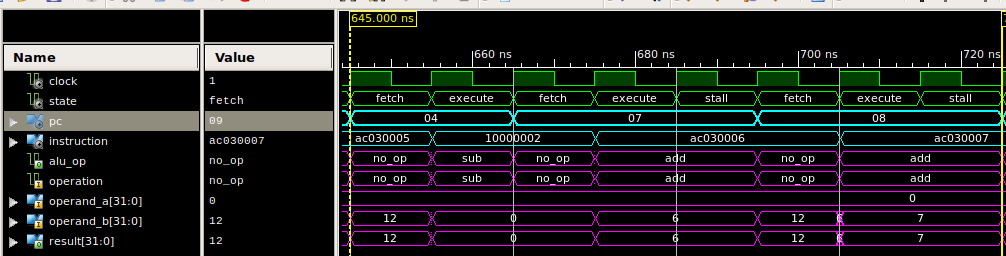
\includegraphics[width=\textwidth]{img/isim}
    \caption{Showing ALU-related signals while \textit{ISim} simulates the instructions\\
        \texttt{beq \$0, \$0, 2}\\
        \texttt{sw \$3, 6(\$0)}\\
        \texttt{sw \$3, 7(\$0)}
    }
    \label{fig:isim}
\end{figure}

\subsubsection{On the FPGA}
After passing all the tests of \texttt{tb\_MIPSProcessor},
the same program was adapted to make it compatible with the \textit{hostcomm} tool.
The \textit{MIPSSystem} was synthesized and a bitfile was created.
After uploading the bitfile, program and data to the FPGA,
the processor was started then stopped after a short while.
The data memory was read back and inspected,
and we could see that it matched the expected output from the tesbench.
Figure \ref{fig:hostcomm} shows a screenshot of this.

\begin{figure}[p]
    \centering
    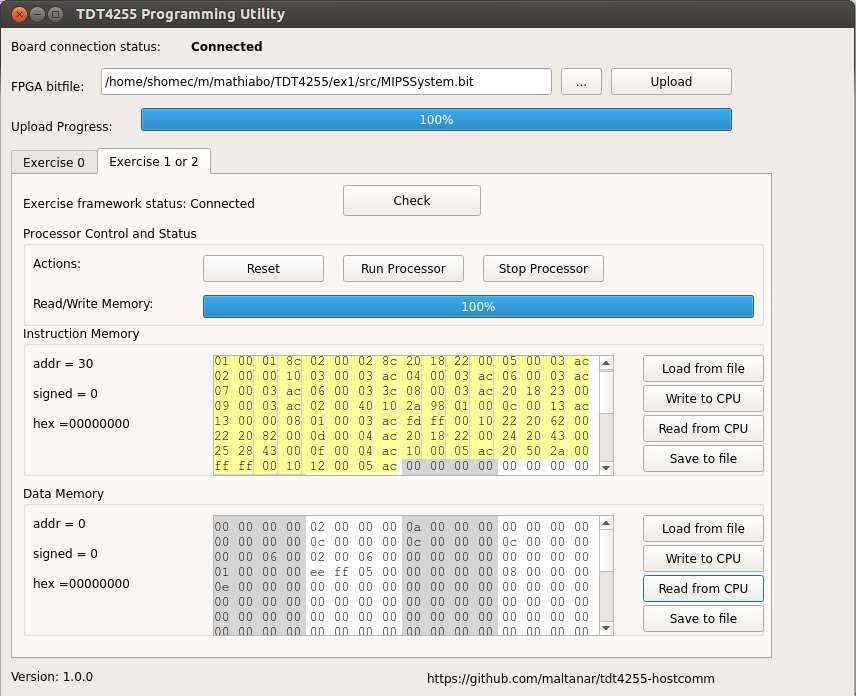
\includegraphics[width=\textwidth]{img/Hostcomm}
    \caption{\textit{hostcomm} after running the processor on the FPGA. The values in the data memory has been read from CPU.}
    \label{fig:hostcomm}
\end{figure}

